\section{Maquettes de l'IHM} 

	\subsection{Client}
	
		\subsubsection{Liste des clients}
		Cette fenêtre permet de consulter la liste des clients de l'agence et d'effectuer des recherches dans cette liste. Au double-clic sur une ligne, une fenêtre contenant le dossier client correspondant s'ouvre. \\
		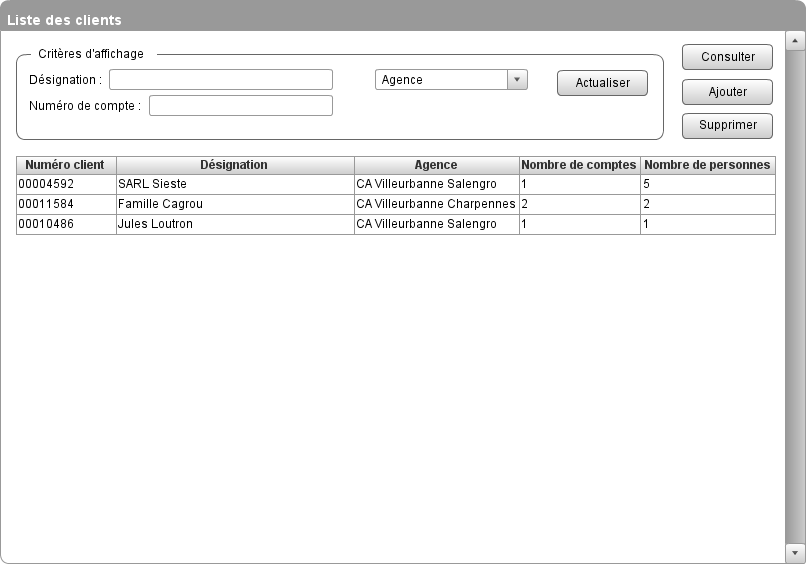
\includegraphics[width=\linewidth]{IHM/Liste_Clients.png}
		
		\newpage		
		
		\subsubsection{Dossier client}
		Lorsque l'on ouvre un dossier client, on accède à ses informations générales (situées en haut de la page). La page contient également 3 onglets : bilan par personne, produits et relation banque-client. Par défaut le premier onglet est sélectionné. \\
		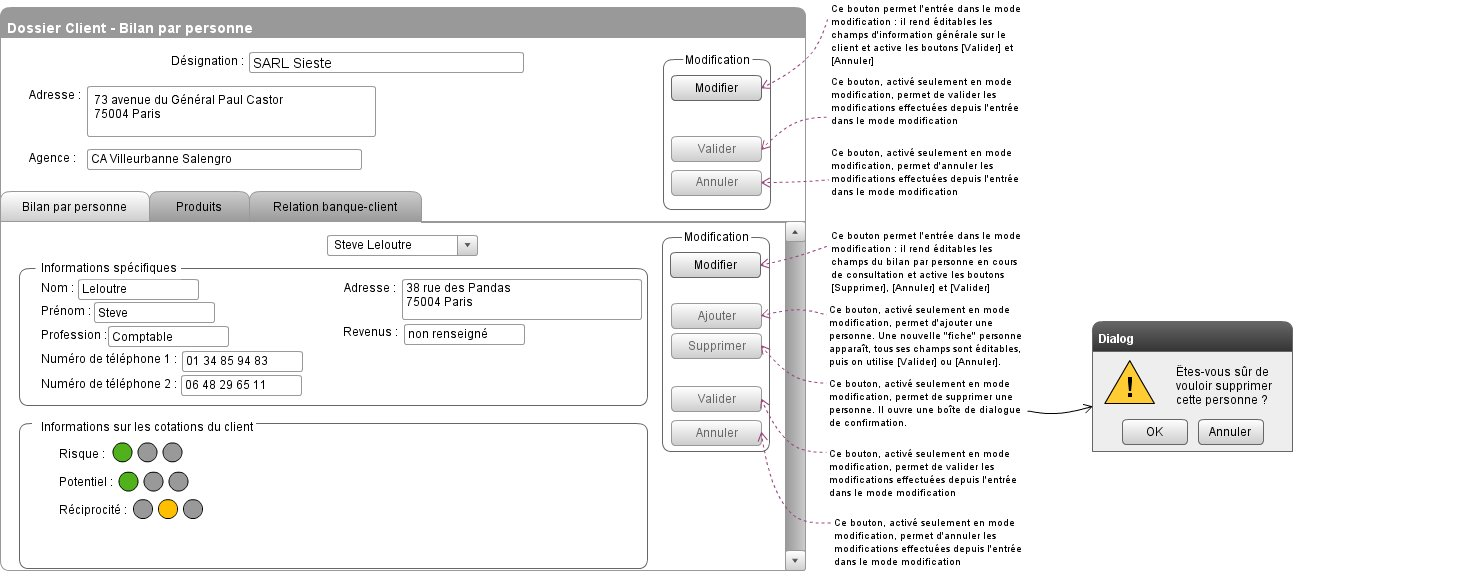
\includegraphics[scale=0.45, angle=90]{IHM/IHMclient1.jpg}
		
		\paragraph*{}
		Ce schéma montre le deuxième onglet. \\
		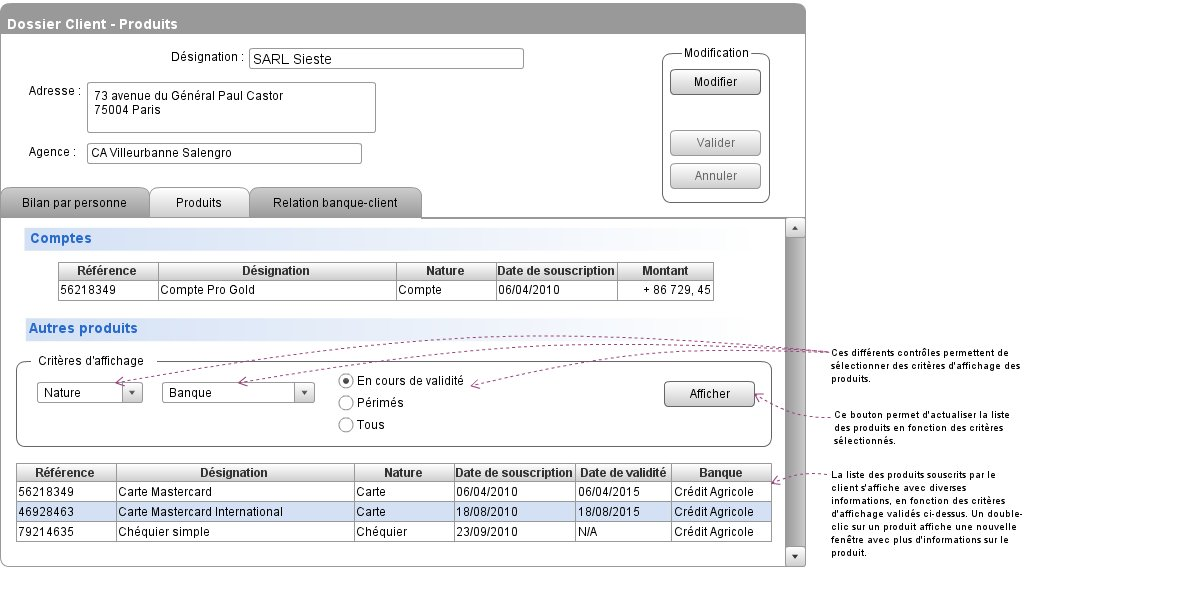
\includegraphics[width=\linewidth]{IHM/IHMclient2.jpg}
		
		\paragraph*{}
		Ces 4 schémas montrent le troisième onglet, qui contient un menu avec 4 options. \\
		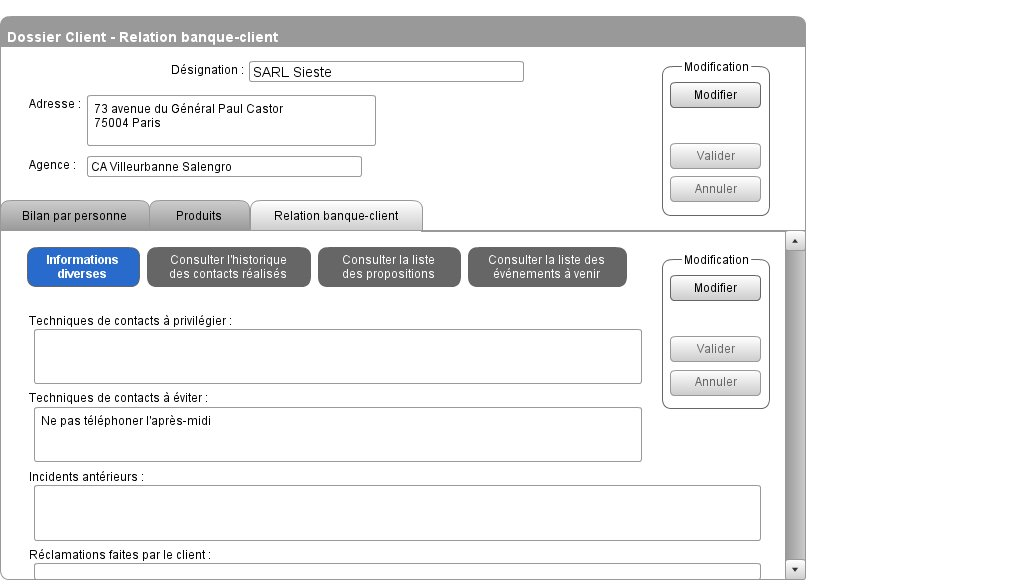
\includegraphics[width=\linewidth]{IHM/IHMclient3.jpg} \\
		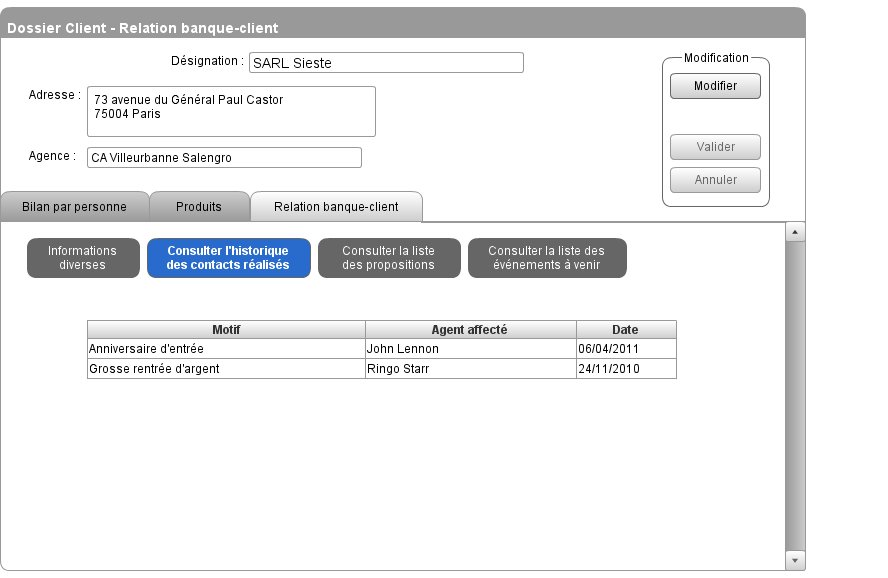
\includegraphics[width=\linewidth]{IHM/IHMclient4.jpg} \\
		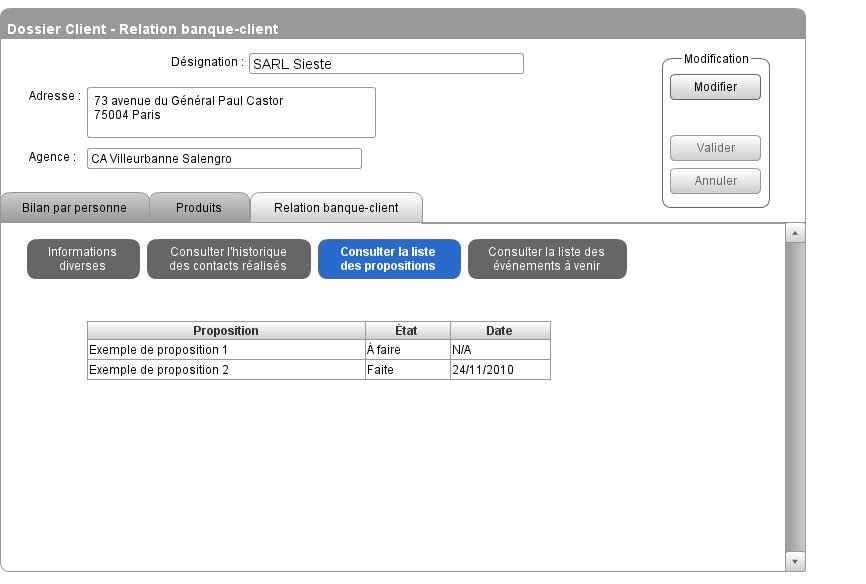
\includegraphics[width=\linewidth]{IHM/IHMclient5.jpg} \\
		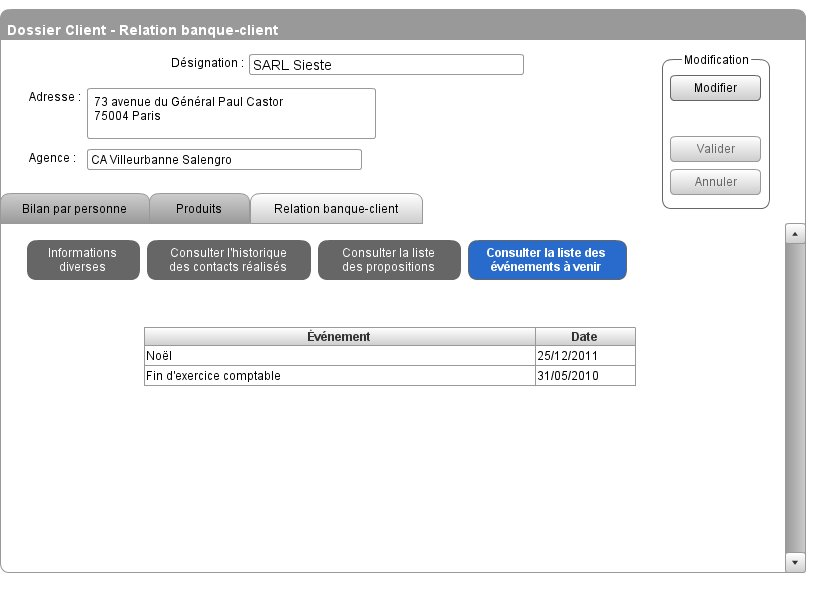
\includegraphics[width=\linewidth]{IHM/IHMclient6.jpg} 
		
	\newpage
		
	\subsection{Contact}
	
		\subsubsection{Liste des contacts}
		Cette fenêtre permet de consulter la liste des contacts de l'agence et d'effectuer des recherches dans cette liste. Au double-clic sur une ligne, une fenêtre contenant les détails du contact correspondant s'ouvre. \\
		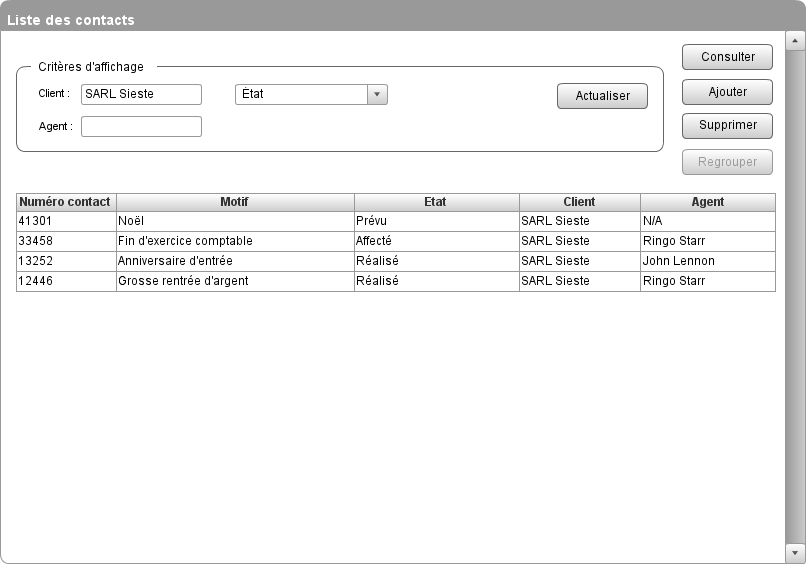
\includegraphics[width=\linewidth]{IHM/Liste_Contacts.png}
		
		\subsubsection{Détail d'un contact}
		Cette fenêtre permet de consulter les détails d'un contact. \\
		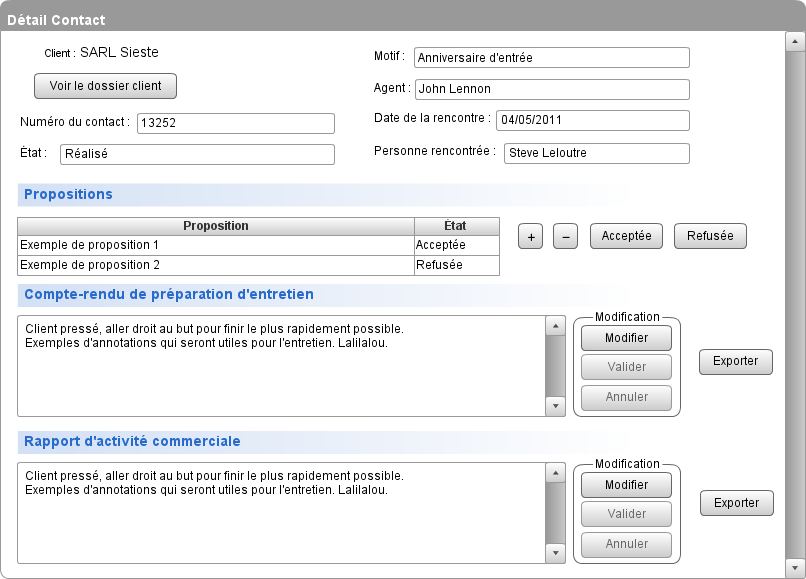
\includegraphics[width=\linewidth]{IHM/Detail_Contact.png}
		
		\newpage
		
	\subsection{Agenda}
		Cette fenêtre permet de consulter l'agenda des agents de l'agence, de créer des plages agenda, de prendre des rendez-vous, de les modifier ou les annuler. \\
		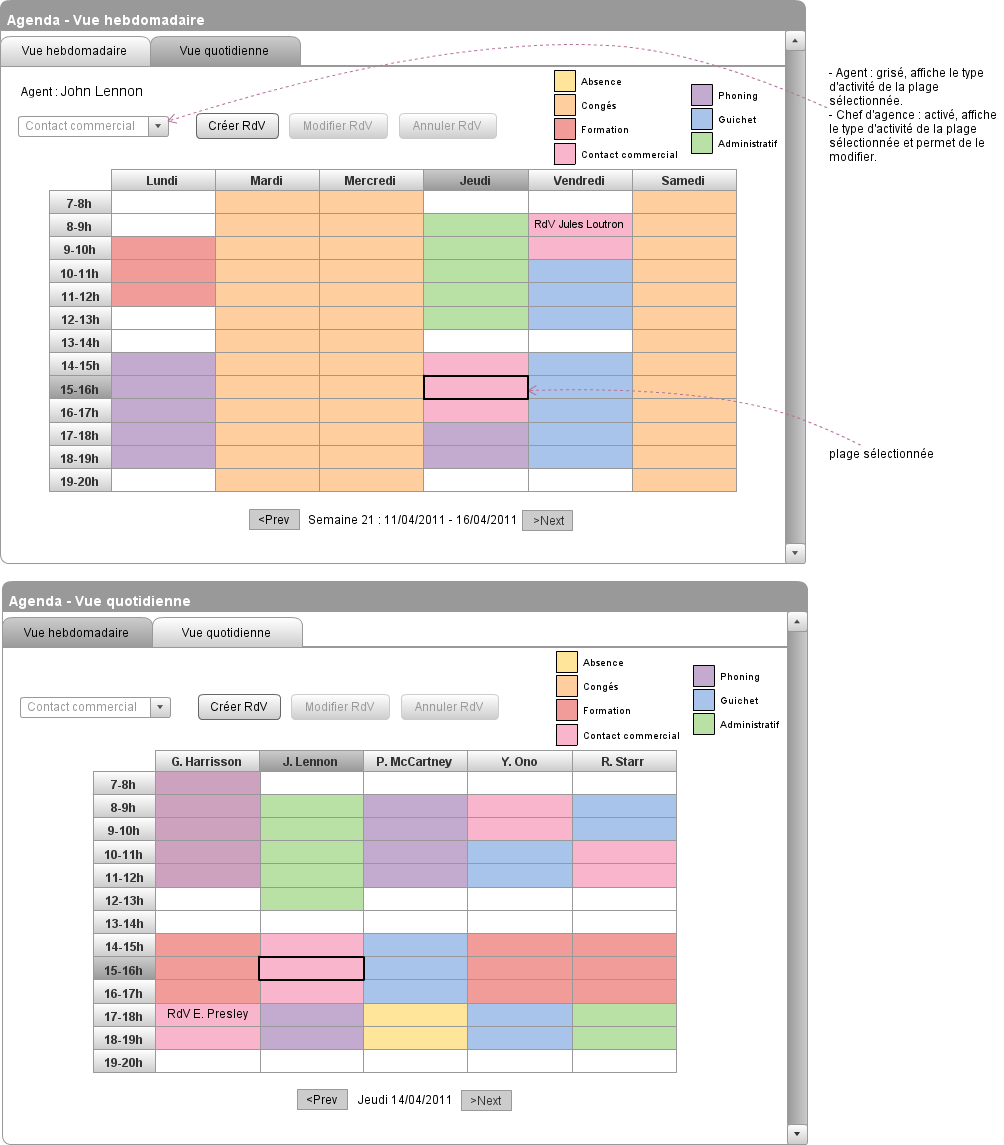
\includegraphics[width=\linewidth]{IHM/Agenda.png}
		
		\newpage